\chapter{SIMULATION OF CONTINUOUS PROCESSES}

This chapter introduces the principles of Euler integration and the method adopted to
couple different subprocesses without transgressing the rules of Euler integration. It is
based on the work of van Kraalingen (1991). A basic knowledge of the state variable
approach, as it is used in continuous simula\-tion, is assumed (see e.g. van Kraalingen,
1991; Penning de Vries \& van Laar, 1982; de Wit \& Goudriaan, 1978).

Various integration methods can be used in the simulation of continuous systems, ranging
from simple rectangular integration (Euler) to higher order integration algorithms 
(trap\-ezoidal, Runge-Kutta, etc.), possibly with a variable time step. From the point of 
view of program structure, a program that accommodates Euler integra\-tion only, is less 
compli\-cated and easier to understand than one accommodating higher order methods of 
integra\-tion. However, this less complicated structure requires changes to be made in the
integration section of the simulating subroutines to allow higher order integration methods
to be used (see Rappoldt \& van Kraalin\-gen 1990). The simulation of crop growth in
FORTRAN often uses Euler integration with a fixed time step (i.e. 1 day) because it
makes the program structure is less complicated and more understandable. Figure \ref{fig:euler}
shows the correct order in which calculations should be executed when Euler integration
is used:

\begin{figure}[p]
% Fig 3.1
\centering
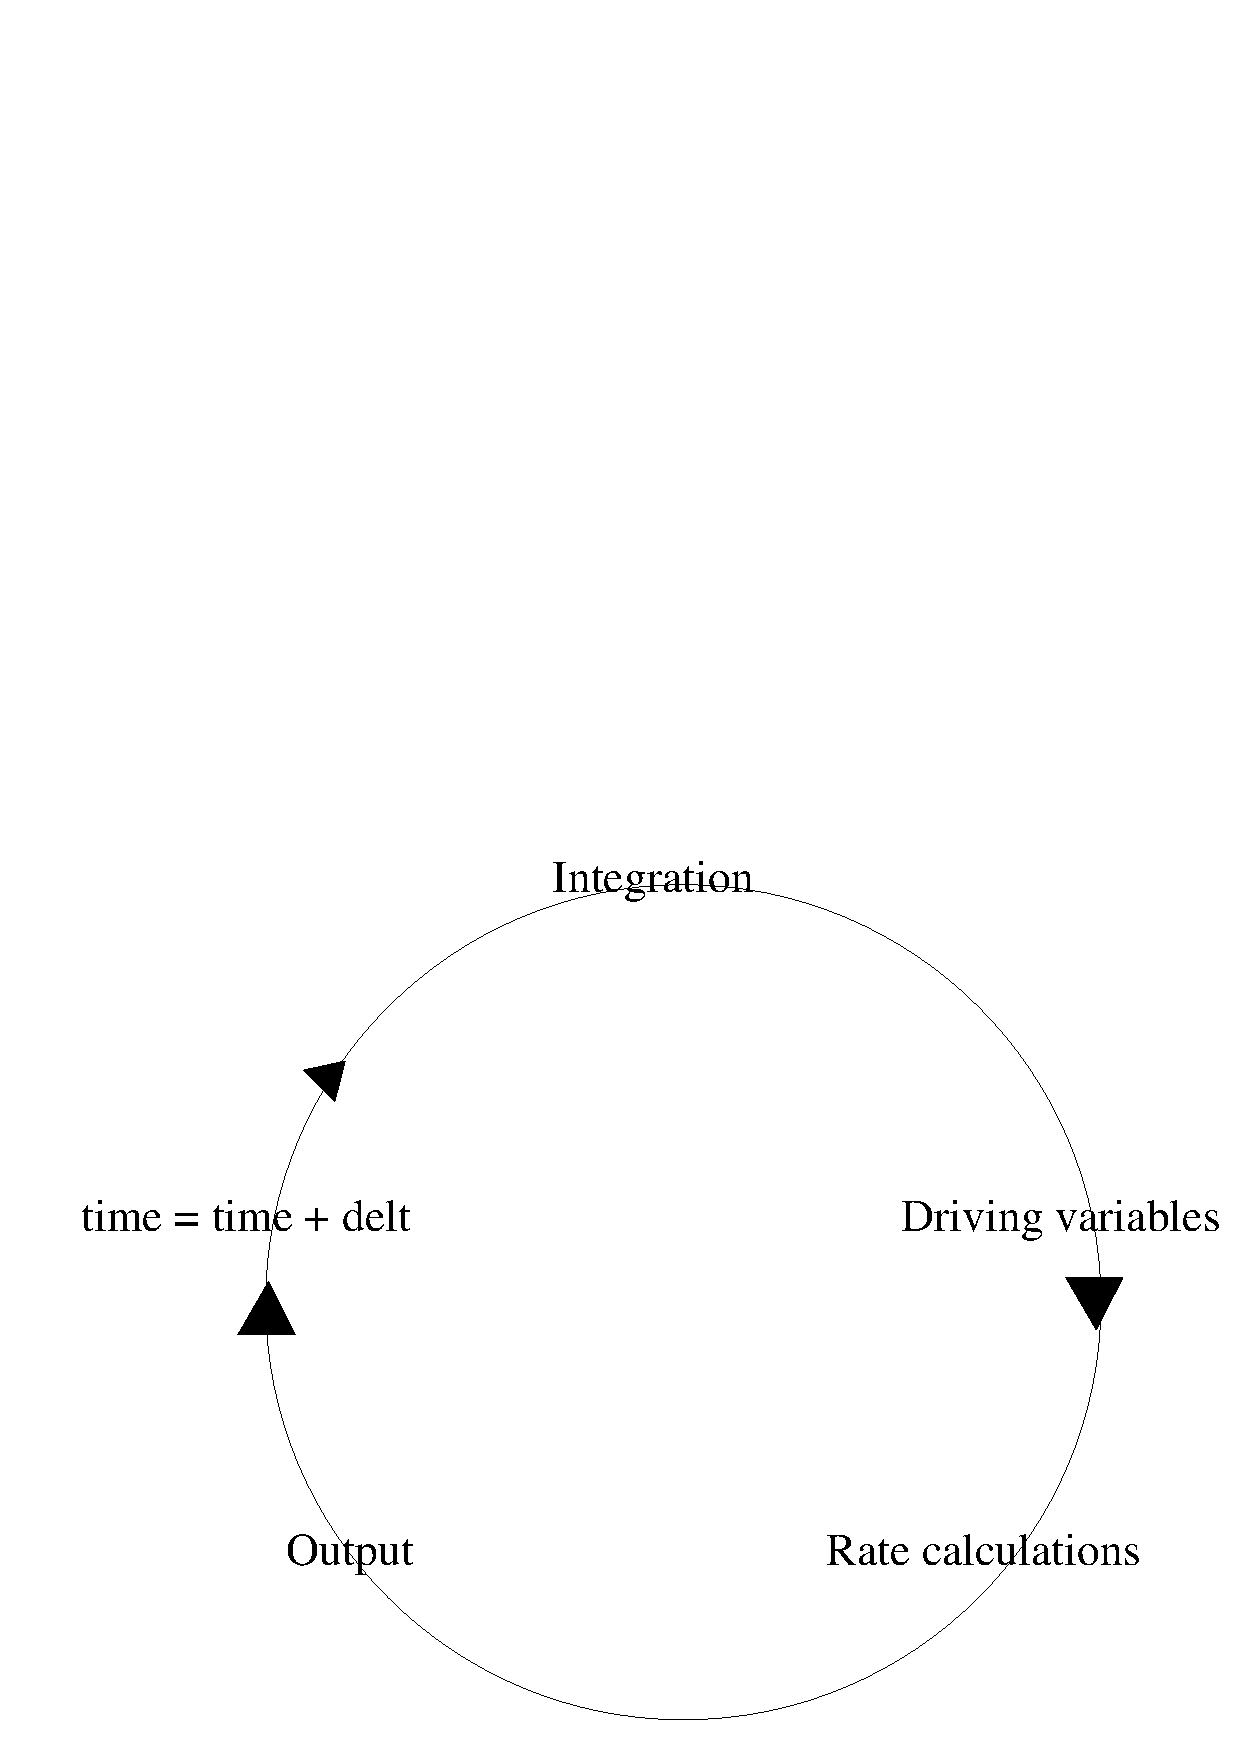
\includegraphics[width=140mm]{\FigDir/FSE0.pdf}
\caption{Order of calcu\-lations when simulat\-ing con\-tinuous systems using Euler 
         inte\-gra\-tion (van Kraalingen, 1991)}
\label{fig:euler}
\end{figure}

Note that in this sequence, at the point where output is generated, state variables and rates
of change correspond to the time for which they were calculated. 

In theory, the sequence in which various state variables are updated, is not important
because their values should not depend on each other but should be fully determined by
the rate variables. In practice, however, state variables may sometimes be derived from
other state variables (e.g. root/shoot ratio or total weight of leaves equals weight of dead
leaves plus weight of green leaves). It is important to put the state calcula\-tions and rate
calculations in the right order.

To ensure that the results of the simulation are correct, the different types of calculations
(integration, driving variables and rate calcula\-tions) should be strictly separated. All states
should be updated, then all driving variables should be calculat\-ed, after which all rates of
change can be determined. If this rule is not applied rigorous\-ly, there is a risk that some
rates will pertain to states at the current time whereas others will pertain to states from
the previous time step.

Since the calculations of rates and states cannot be mixed during a time step but should be
executed separately, all the state calculations have to be merged into one block as do all
the rate calculations. Often, different subprocesses are interacting. In many cases these
interactions among the subprocesses are only weak. The water content at different depths
in the soil, for example, is needed for the plant/soil system in the plant submodel. This is
then used to deter\-mine water uptake for transpiration in dependence of rooting depth. The
submodels for the plant and soil water thus share a limited amount of information,
however, they may contain very detailed descriptions of plant growth and soil moisture
redistribution with many different rate and state calcula\-tions.

In view of the above, it is not a good solution to combine all the state calculations from
the different subprocesses into one large program section and all the rate calculations in
another. But it is feasible to separate the state and rate calculations within the subprocess
descriptions and have a calling program decide which of the two to execute. With this
method, the states can be calculated separately from the rates, whereas rates and states
pertaining to the same subprocess are within the same subprogram. This technique is also
discussed by van Kraalingen and Rappoldt (1989).

This concept of 'task-controlled execution' is illustrated in figure \ref{fig:fse_struct)} The program lines
of the plant and soil water subprocesses are separated into rate and state sections and only
one of these is executed during a single call. Note that this program structure performs
the calculations in exactly the same order as the circle given in figure \ref{fig:euler}.

So far, the initialization of the states variables or where to enter the simula\-tion circle and
where to leave it, is not discussed, (see figure \ref{fig:euler}). It is convenient to leave the circle
somewhere between time update and integration, because there the time and correspond\-ing 
rates have been written to the output device and after the time update it seems logical
to check whether the finish time (end date of simulation) has been exceeded or whether
further simulation is required. Consequently, the circle should also be entered between
time update and integration.

The most conve\-nient way to initialize the subprocesses is to have this operation controlled
by the main program. This makes reruns possible, because in the main  program the
whole model can be reset to its initial state and be run again, with different weather data
for instance. These refinements to figure \ref{fig:euler} are shown in figure \ref{fig:fse_order}.

\begin{figure}[p]
%fig 3.2
\centering
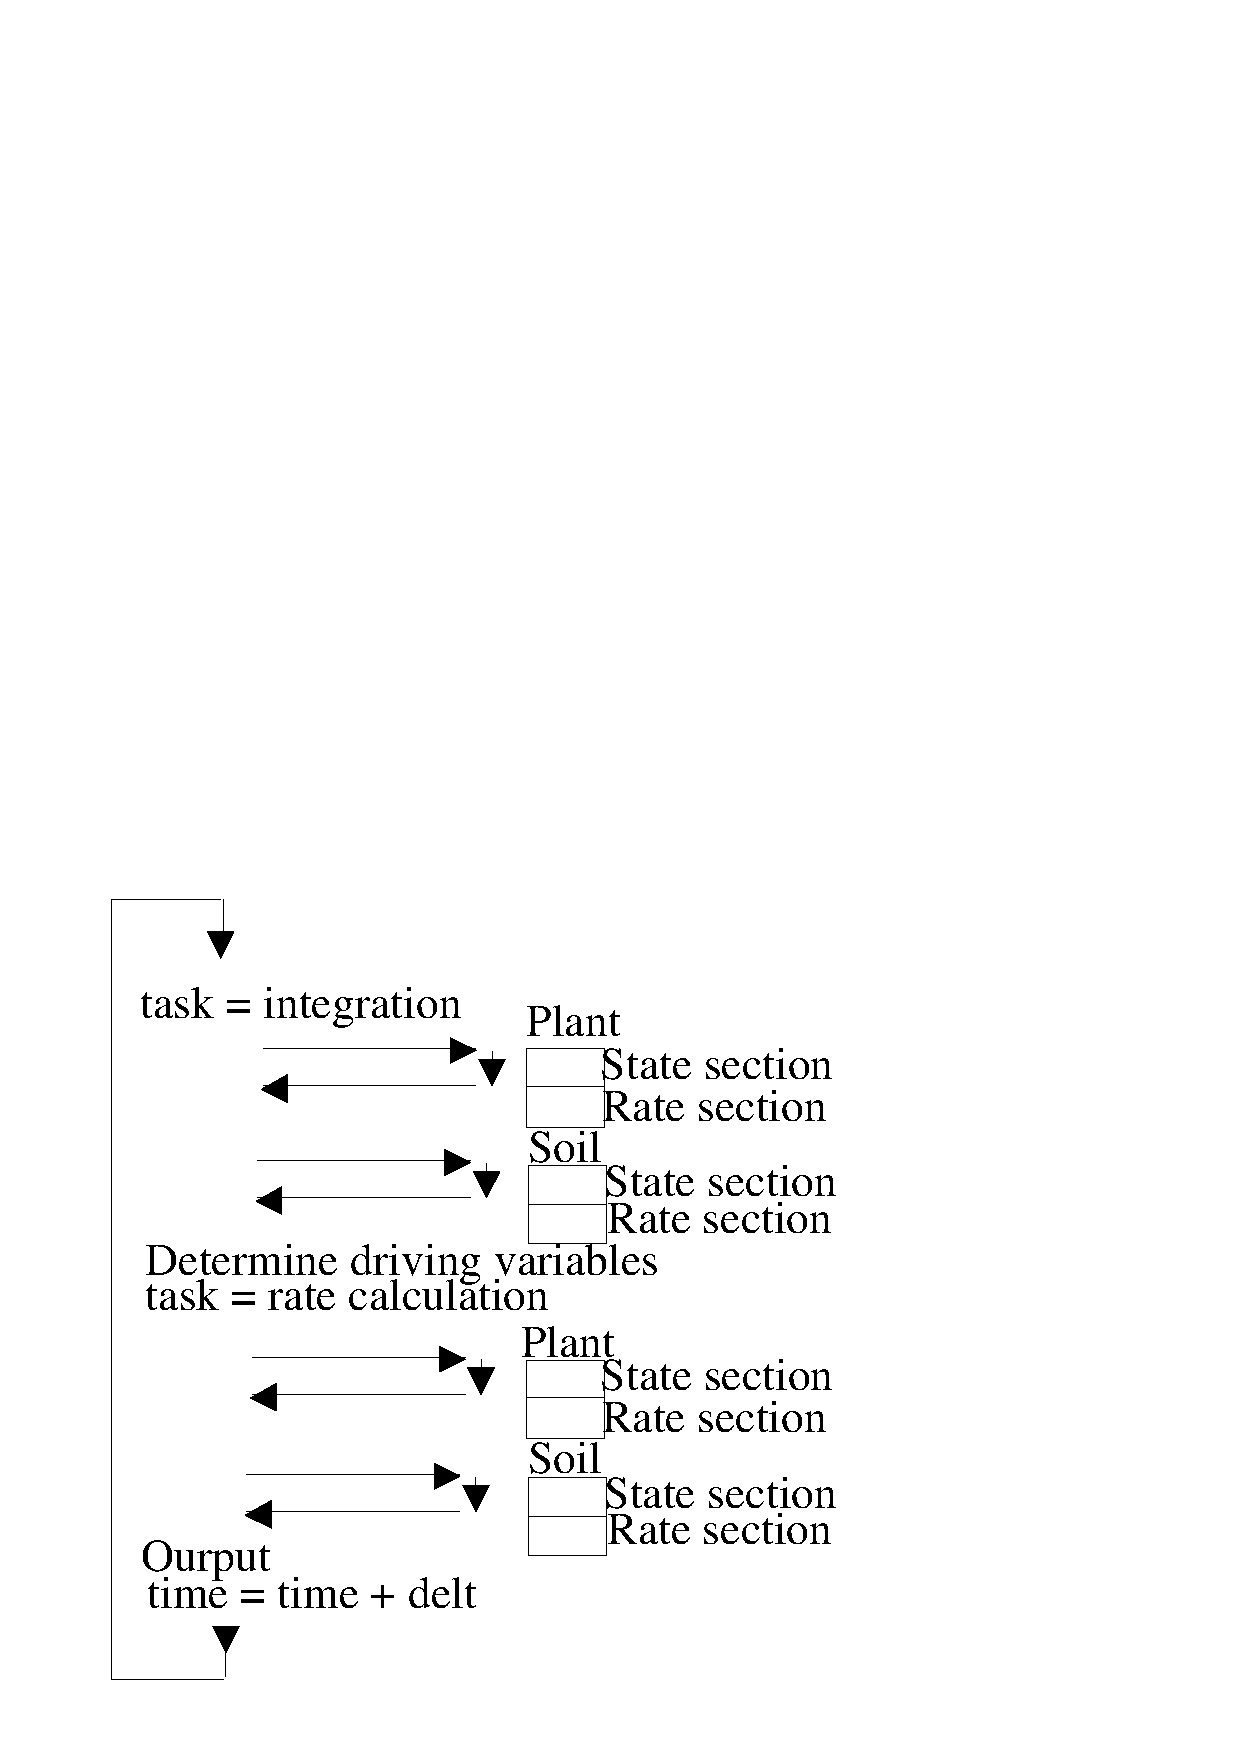
\includegraphics[width=140mm]{\FigDir/FSE1.pdf}
\caption{Gen\-er\-al s\-t\-ruc\-t\-ure for in\-corporating several subprocesses 
containing integra\-tion and rate cal\-culation into a single simulation model (van Kraalingen,
1991).}
\label{fig:fse_struct}
\end{figure}

The question mark between time = time+delt and integration in figure \ref{fig:fse_order}, indicates the
point at which it is decided whether or not to execute another time step. If the decision is
"no", the model proceeds to the terminal section; if it is "yes" the circle is run once
more. After proceeding to the terminal section, it must be decided whether a rerun is
required. If the decision is "yes" the model has to be re-initialized and a new simula\-tion
run is started.

As shown in figure \ref{fig:fse_order}, the modularity of the subprocess descriptions is preserved by
introducing the concept of task-controlled execution (the calling program decides what the
subroutine should do: either integration or rate calculation). To be able to do reruns, the
various subprocess descriptions that can also be driven by the task variable have to be
initialized externally, and some terminal calculations (e.g. harvest index) have to be done.
Therefore, a subprocess in the program should recognize four different tasks: {\bf Initializa\-tion}, 
{\bf Integration}, {\bf Rate Calcula\-tion} and {\bf Terminal Calcula\-tion}.

\begin{figure}[p]
%Fig. 3.3 
\centering
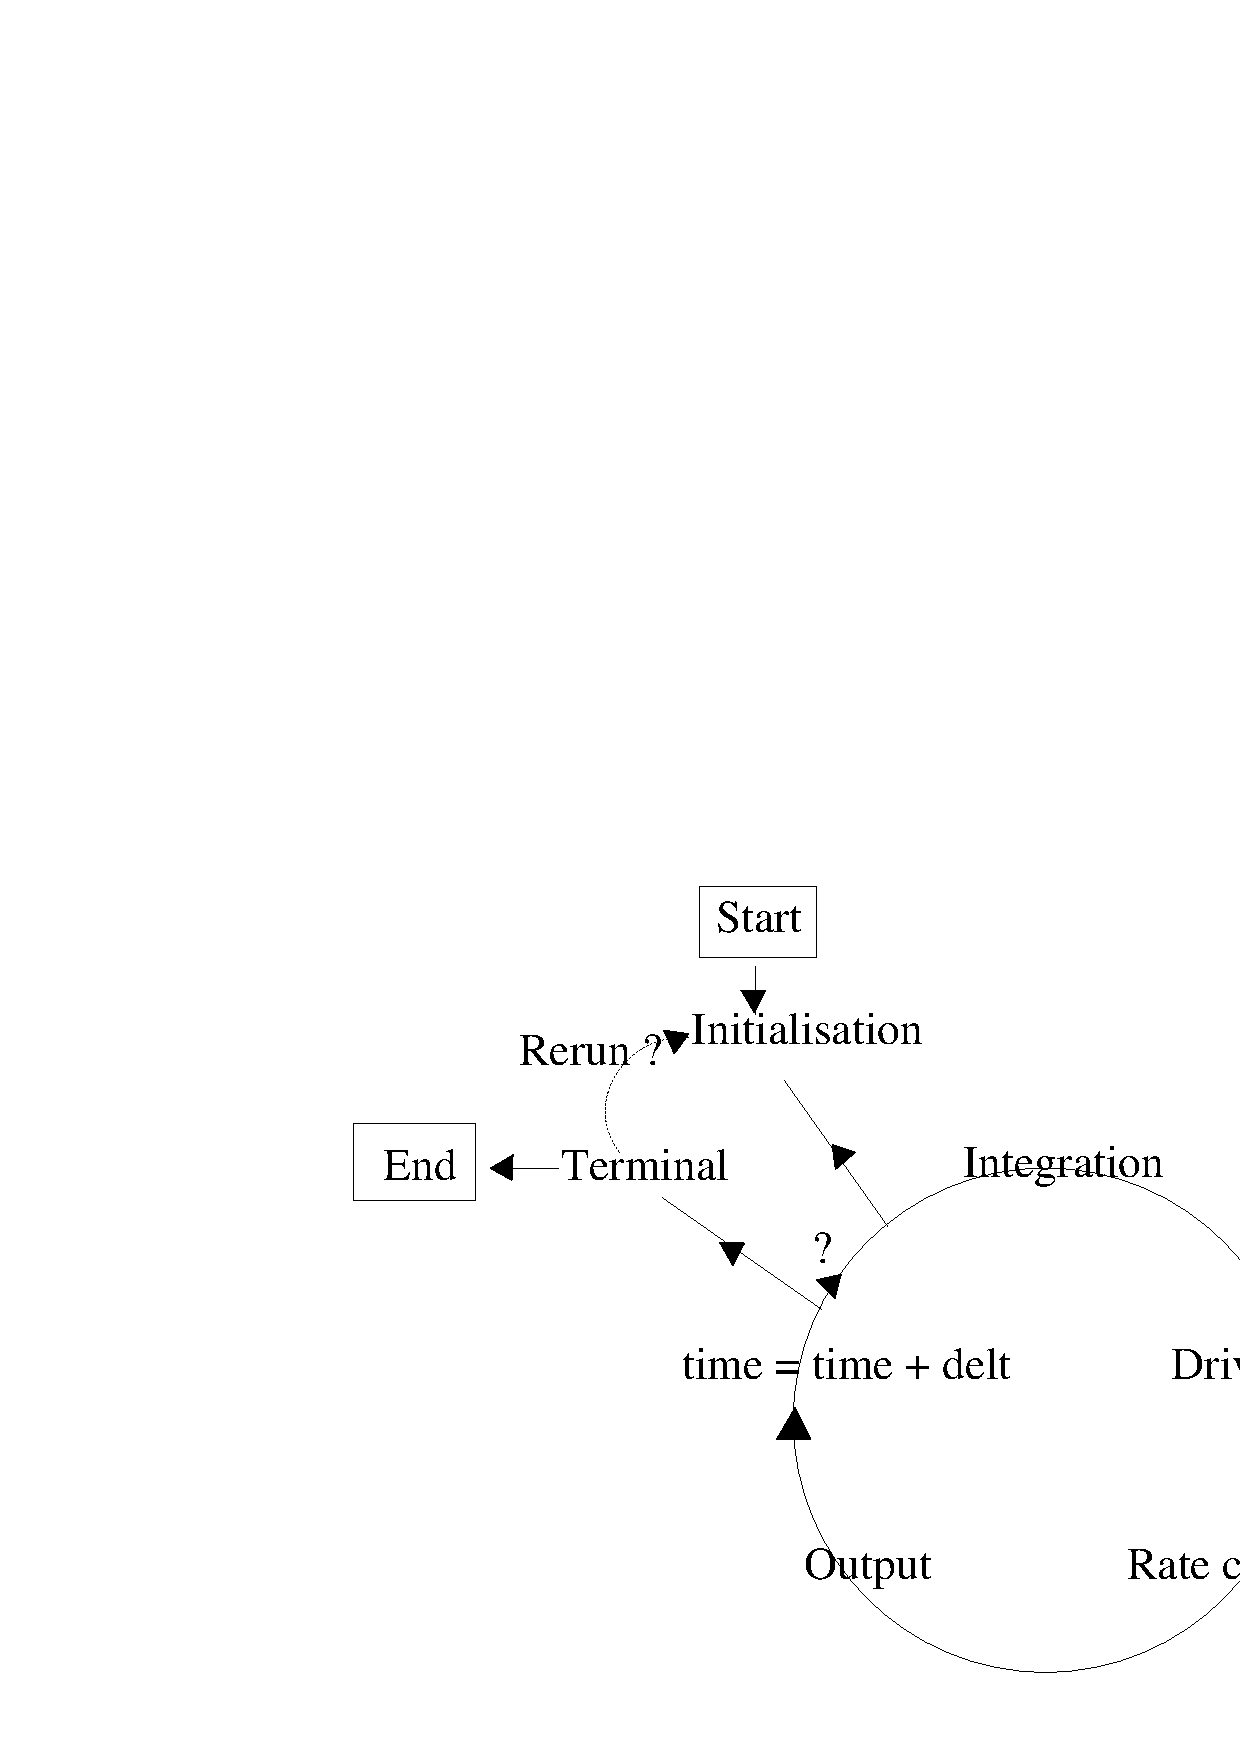
\includegraphics[width=140mm]{\FigDir/FSE2.pdf}
\caption{Order of cal\-cu\-la\-tions when simulating continuous systems using Euler
integra\-tion, illustrating where to enter and leave the circle and how reruns
are implemented (van Kraalingen, 1991)}
\label{fig:fse_order}
\end{figure}

A consequence of this structure, the first step after initialization is integration. This does
no harm if the rates have been set to zero explicitly, so that the first integration has no
effect on the value of the states. In practice this means incorporat\-ing many rate assign\-ments 
which are set equal to zero into the model. To avoid this, integration can be
skipped if the previous task was initialization (during which the states have been assigned
values anyway). The subsequent rate calculation will then use the state variables to
initialize the rates of change.

It should be noted that there exists a clear distinction between the use of the Euler
integration and the Gaussian integration, which is used extensively in chapters five and
six. See also Appendix 1. The Euler integration is used to integrate the process\-es on a
larger scale than the Gaussian method. The Euler integration as discussed above, is used
to integrate all the crop growth processes over the growing period (i.e. all the time steps
executed), while the Gaussian integration is used to integrate the individual processes over
for example depth, or one day (i.e one time step). 

The integration of the rate variables over time in order to get the state variables, is 
implemented as follows.

\begin{equation}
Q _{t~} =~Q _{t-1} ~+~\Delta Q _{t} \,\Delta t
\end{equation}

Where:\\
\begin{tabularx}{\textwidth}{llXr}
 Qt &:& State variable at time step t    &   [unit]\\
 $\Delta$Q$_{{\rm t}}$ &:& Rate variable at time step t   &    [unit d$^{{\rm -1}}$]\\
 $\Delta$t &:& Time step   &    [d]\\
\end{tabularx}
